\Sec{Análise e Projeto}

\Subsec{Operações Aritméticas}

As operações aritméticas realizadas pela ALU incluem somas e subtrações entre operandos de 4 \textit{bits}, além de operações de incremento e decremento. Essas operações utilizam um \textit{bit} adicional, \textit{carry-in} ($CBi$), que permite expandir a funcionalidade aritmética da ALU ao incorporar o conceito de “vai-um” em somas e “empréstimo” em subtrações.

\Subsubsec{Adição}

A operação de adição soma os valores dos operandos $X$ e $Y$, incluindo o valor do \textit{carry-in} ($CBi$), resultando num número de 4 bits. Se o resultado ultrapassar o valor máximo representável em 4 \textit{bits}, ocorre um \textit{carry-out}, indicado pela \textit{flag} $CBo$. A \textit{flag} $OV$ (overflow) é ativada quando o resultado excede a capacidade de representação de números com sinal, indicando um erro de estouro de valor. A adição pode ser representada logicamente pela expressão:

\begin{figure}[H]
    \centering
    \tcbox{\large $X + Y + CBi = R$}
    \caption{Expressão da Adição}
\end{figure}

\Subsubsec{Subtração}

A operação de subtração calcula a diferença entre os operandos $X$ e $Y$, considerando o bit \textit{carry-in} ($CBi$) como \textit{borrow-in} ou empréstimo. Essa operação gera as mesmas \textit{flags} que a adição, com uma diferença: a \textit{flag} $CBo$ aqui sinaliza um \textit{borrow-out}, indicando que foi necessário um “empréstimo” para a operação. A \textit{flag} $OV$ indica ativa quando o resultado está fora dos limites de representação de números com sinal. A expressão lógica da subtração é dada por:

\begin{figure}[H]
    \centering
    \tcbox{\large $X - Y - CBi = R$}
    \caption{Expressão da Subtração}
\end{figure}

\newpage

\Subsubsec{Incremento}

A operação de incremento adiciona o valor de $X$ ao \textit{carry-in} ($CBi$), aumentando o operando em uma unidade quando $CBi$ = 1. Durante o incremento, o bloco $Yor0$  é ativado, desconsiderando o valor de $Y$ (todos os \textit{bits} de $Y$ são configurados para zero). O incremento gera as mesmas \textit{flags} que a adição, com exceção de que o \textit{carry-in} é adicionado diretamente ao operando $X$. A expressão lógica que representa o incremento é:

\begin{figure}[H]
    \centering
    \tcbox{\large $X + CBi = R$}    
    \caption{Expressão do Incremento}
\end{figure}

\Subsubsec{Decremento}

A operação de decremento subtrai o \textit{carry-in} ($CBi$) de $X$, diminuindo o valor do operando em uma unidade, caso $CBi$ = 1. Nesta operação, o bloco $Yor0$ também é ativado, eliminando a influência do operando $Y$. As \textit{flags} geradas pelo decremento são as mesmas da subtração, com a \textit{flag} $CBo$ indicando um \textit{borrow-out}, se houver necessidade de “empréstimo” durante a operação. A expressão lógica para o decremento é:

\begin{figure}[H]
    \centering
    \tcbox{\large $X - CBi = R$}
    \caption{Expressão do Decremento}
\end{figure}

\Subsec{Operações Lógicas}

Além das operações aritméticas, a ALU é projetada para realizar operações lógicas com o $X$ (e com $Y$ caso seja um NAND). O Módulo Lógico, para além de retornar o resultado das operações, retorna o bit que desaparece nas operações de deslocamento (LSR, ASR, LSL).

\Subsubsec{Deslocamento Lógico à Direita (LSR)}

O deslocamento lógico à direita é a operação binária que move todos os 4 \textit{bits} uma posição para a direita, preenchendo a posição restante na extremidade esquerda com zero. A expressão lógica para o deslocamento lógico à direita é:

\begin{figure}[H]
    \centering
    \tcbox{\large $X >>> 1$}
    \caption{Expressão do LSR}
\end{figure}

\Subsubsec{Deslocamento Aritmético à Direita (ASR)}

Diferentemente do deslocamento lógico à direita, o deslocamento aritmético à direita é uma operação binária que move todos os \textit{bits} de um número para a direita por uma certa quantidade de posições, mas preservando o \textit{bit} de sinal (o \textit{bit} mais à esquerda). A expressão lógica para o deslocamento aritmético à direita é:

\begin{figure}[H]
    \centering
    \tcbox{\large $X >> 1$}
    \caption{Expressão do ASR}
\end{figure}

\Subsubsec{Deslocamento Lógico à Esquerda (LSL)}

O deslocamento lógico à esquerda é uma operação binária que move todos os \textit{bits} de um determinado número para a esquerda por uma certa quantidade de posições, preenchendo a posição restante na extremidade esquerda com zero. A expressão lógica para o deslocamento lógico à esquerda é:

\begin{figure}[H]
    \centering
    \tcbox{\large $X <<< 1$}
    \caption{Expressão do LSL}
\end{figure}

\subsubsection{Operação NAND}

O operador lógico NAND é uma operação booleana que utiliza os operadores AND ($\cdot$) e NOT (¬). Em resumo, esse operador lógico resulta no complemento da operação AND e é representado pela expressão:

\begin{figure}[H] \centering \tcbox{\Large $\overline{X \cdot Y}$} \caption{Expressão do operador NAND} \end{figure}
\newpage

\Subsec{Geração e Descrição das Flags}

\Subsubsec{\textit{Flag} CBo (\textit{Carry}/\textit{Borrow})}

Esta \textit{flag} representa o \textit{carry} de saída da operação de soma ou o \textit{borrow} de saída da operação de subtração. Fica ativa quando o resultado excede o domínio. No âmbito das operações lógicas (LSR, ASR e LSL), a \textit{flag} retorna o valor do \textit{bit} deslocado de X que desaparece do resultado.

\Subsubsec{\textit{Flag}{ OV (\textit{Overflow})}}

Sempre que o resultado de uma operação excede o domínio dos números relativos a \textit{flag} de \textit{overflow} é ativada.

\Subsubsec{\textit{Flag} Z (Zero)}

Esta \textit{flag} fica ativa quando o resultado de uma operação é zero (0).

\Subsubsec{\textit{Flag} P (Paridade)}

Quando o resultado de uma operação tem um número ímpar de 1s a \textit{flag} é ativada.

\Subsubsec{\textit{Flag} GE (\textit{Greater or Equal})}

Esta \textit{flag} tem a função de indicar se o primeiro operando ($X$), é maior ou igual ao segundo operando ($Y+CBi$). A \textit{flag} atua na representação de números relativos e só deve ser considerada quando a operação realizada é uma subtração.

\Subsubsec{\textit{Flag} BE (\textit{Below or Equal})}

Similarmente à \textit{flag} anterior, a \textit{flag} $BE$ tem a função de indicar se o primeiro operando ($X$), é menor ou igual ao segundo operando ($Y+CBi$). Ao contrário da \textit{flag} $GE$, esta \textit{flag} atua na representação de números naturais e só deve ser considerada quando a operação realizada é uma subtração.

\newpage
\Subsec{Diagramas Lógicos}

\Subsubsec{Módulo Aritmético}

\begin{figure}[h]
    \centering
    \tcbox[title=Módulo Aritmético,center title,halign=center,valign=center]{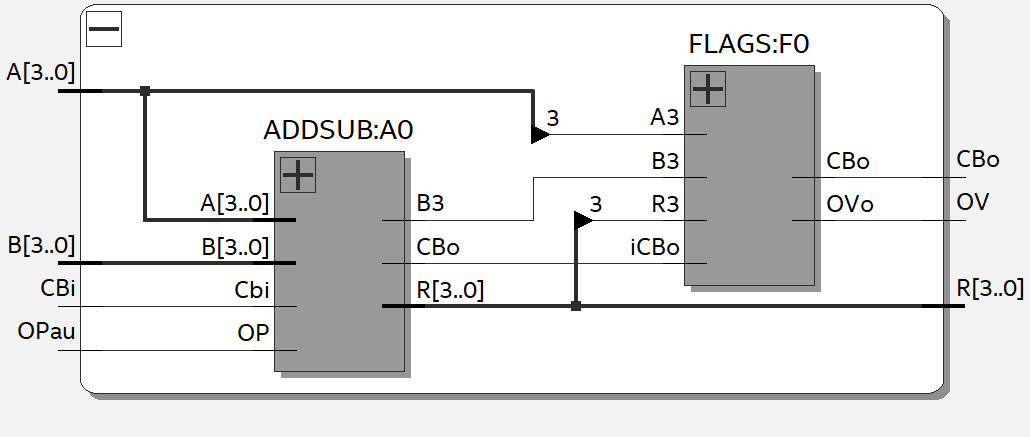
\includegraphics[scale=0.4]{Análise e Projeto/images/AU Module.png}}
    \caption{Diagrama lógico do Módulo Aritmético}
\end{figure}

\begin{figure}[H]
    \centering
    \begin{tcolorbox}[title=Sub-Módulos do Módulo Aritmético,center title,halign=center,valign=center]
        \begin{tcbitemize}[raster columns=2,raster equal height]
            \tcbitem[squeezed title=Módulo Somador/Subtrator,center title,halign=center,valign=center]
                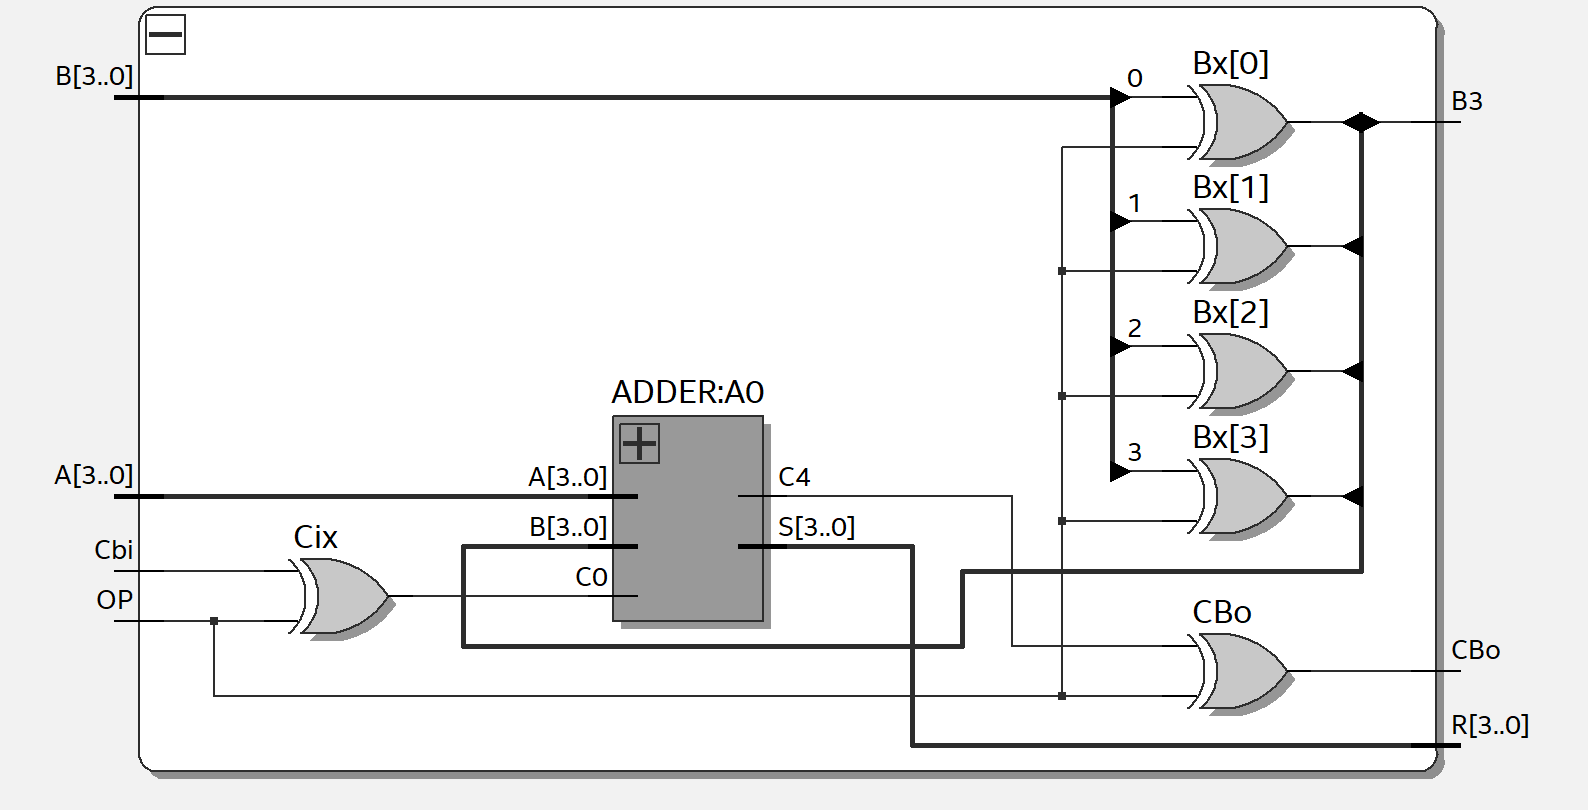
\includegraphics[scale=0.18]{Análise e Projeto/images/Adder Subtractor.png}
            \tcbitem[squeezed title=Módulo Somador de 4 Bits,center title,halign=center,valign=center]
                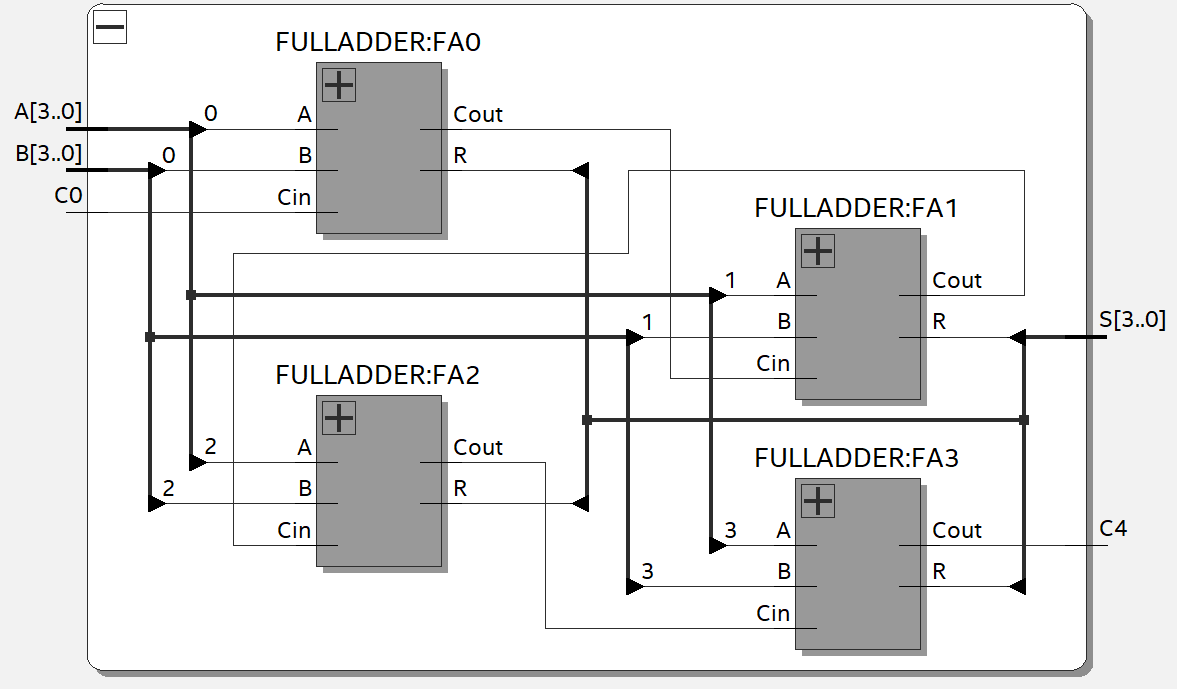
\includegraphics[scale=0.24]{Análise e Projeto/images/Adder.png}
        \end{tcbitemize}
        \begin{tcbitemize}[raster columns=2,raster equal height]
            \tcbitem[squeezed title=Módulo Somador de 1 Bit,center title,halign=center,valign=center]
                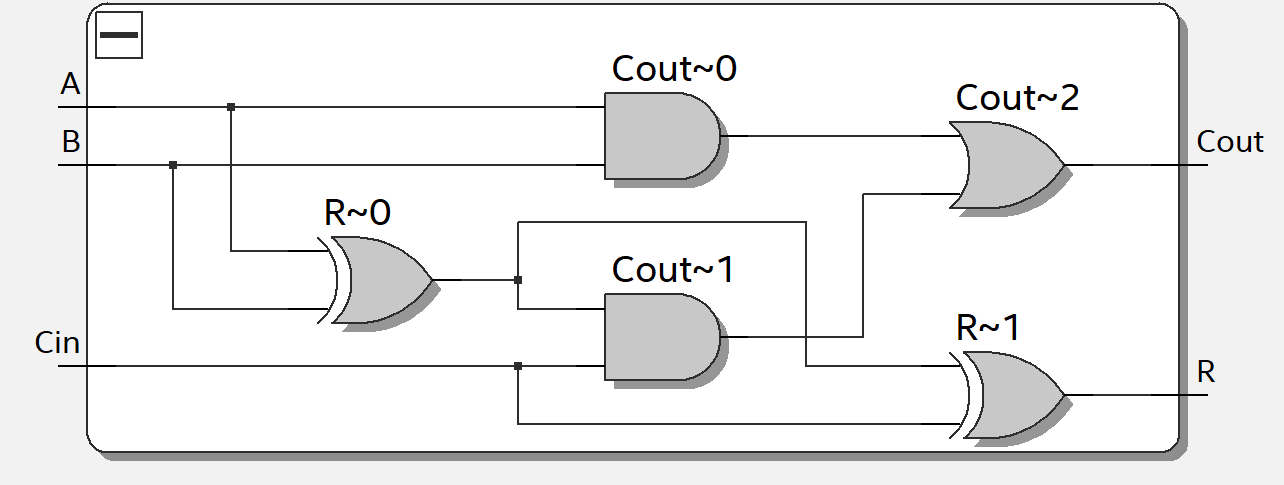
\includegraphics[scale=0.21]{Análise e Projeto/images/Fulladder.png}
            \tcbitem[squeezed title=Módulo \textit{Flags},center title,halign=center,valign=center]
                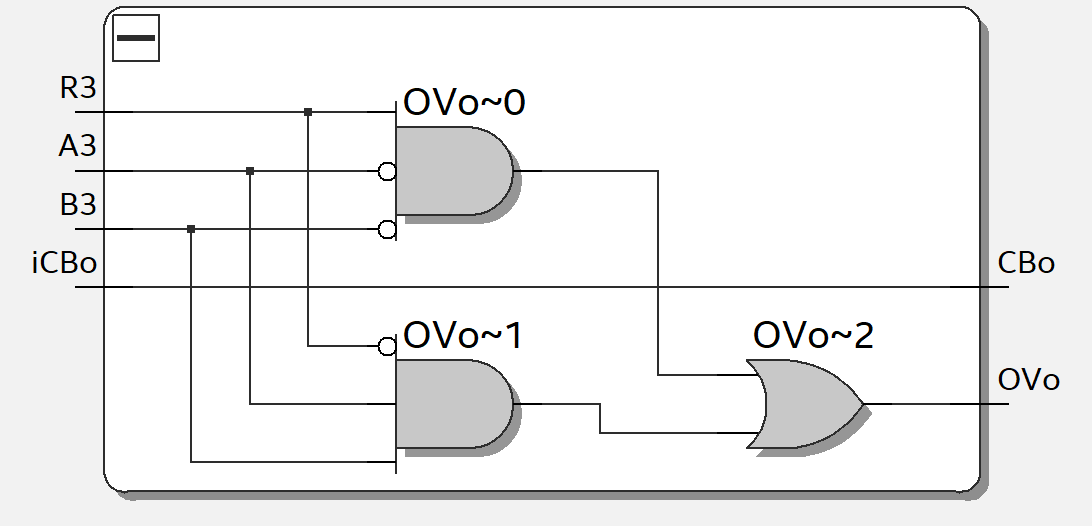
\includegraphics[scale=0.25]{Análise e Projeto/images/AU Flags.png}
        \end{tcbitemize}
    \end{tcolorbox}
    \caption{Sub-Módulos do Módulo Aritmético}
\end{figure}


\Subsubsec{Módulo Lógico}

\begin{figure}[H]
    \centering
    \tcbox[title=Módulo Lógico,center title,halign=center,valign=center]{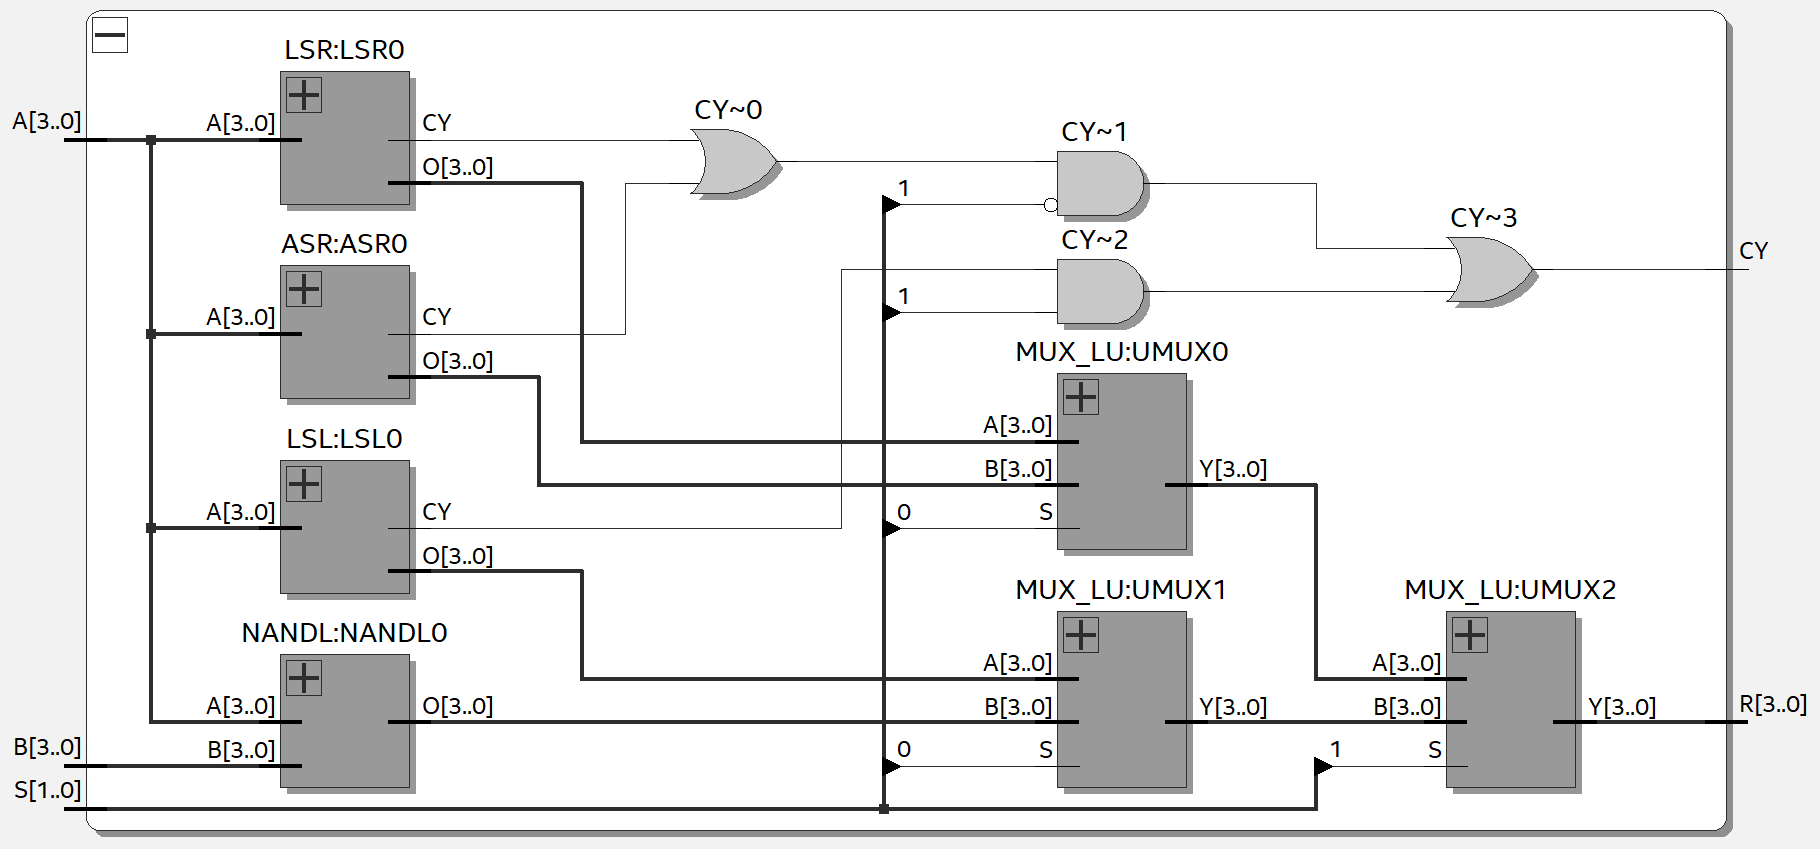
\includegraphics[scale=0.28]{Análise e Projeto/images/LU Module.png}}
    \caption{Diagrama lógico do Módulo Lógico}
\end{figure}

\begin{figure}[H]
    \centering
    \begin{tcolorbox}[title=Sub-Módulos do Módulo Lógico,center title,halign=center,valign=center]
        \begin{tcbitemize}[raster columns=3,raster equal height]
            \tcbitem[squeezed title=Módulo ASR,center title,halign=center,valign=center]
                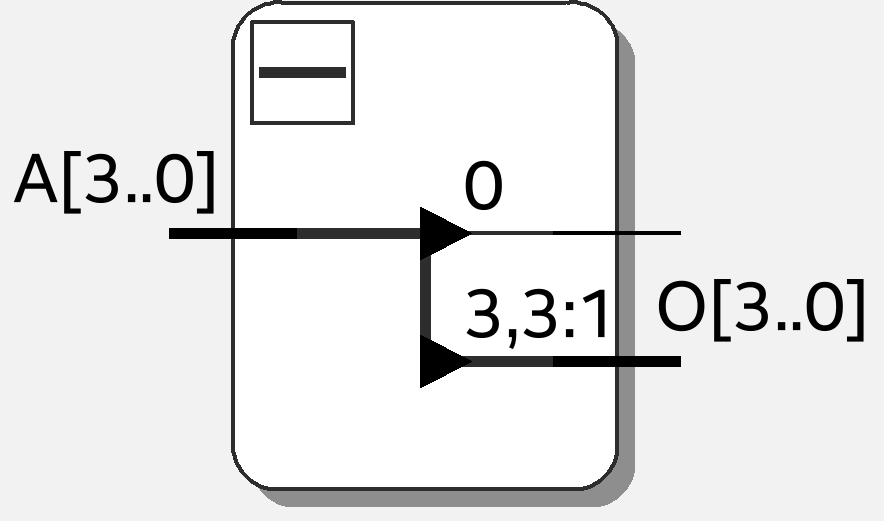
\includegraphics[scale=0.18]{Análise e Projeto/images/ASR.png}
            \tcbitem[squeezed title=Módulo LSR,center title,halign=center,valign=center]
                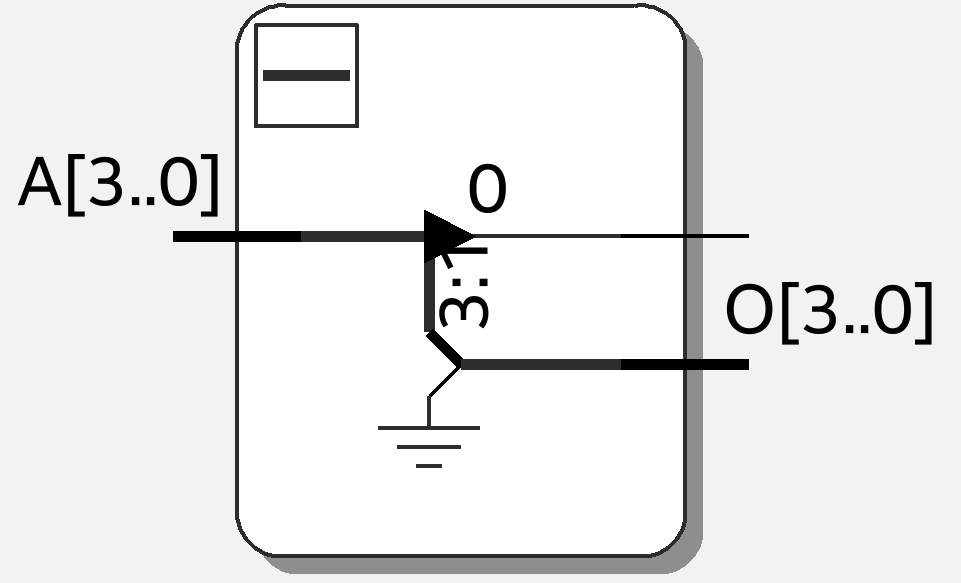
\includegraphics[scale=0.165]{Análise e Projeto/images/LSR.png}
            \tcbitem[squeezed title=Módulo LSL,center title,halign=center,valign=center]
                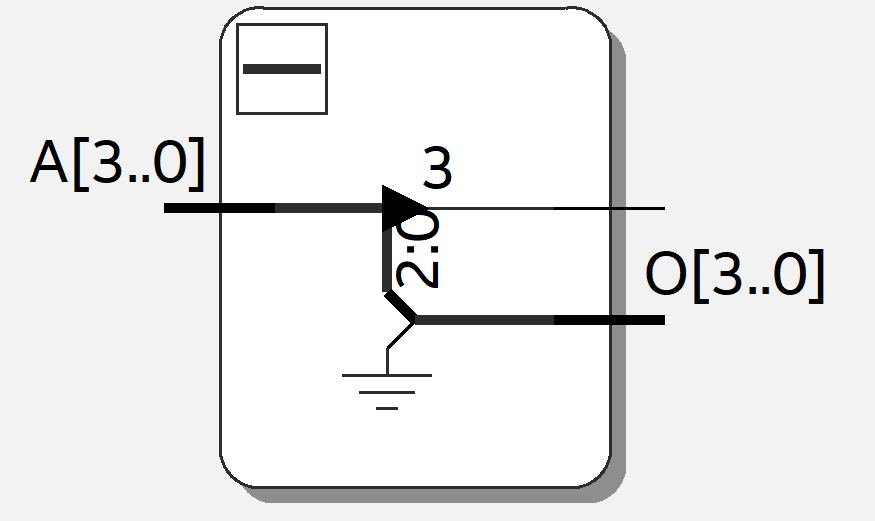
\includegraphics[scale=0.18]{Análise e Projeto/images/LSL.png}
        \end{tcbitemize}
        \begin{tcbitemize}[raster columns=2,raster equal height]
            \tcbitem[squeezed title=Módulo Somador de 1 Bit,center title,halign=center,valign=center]
                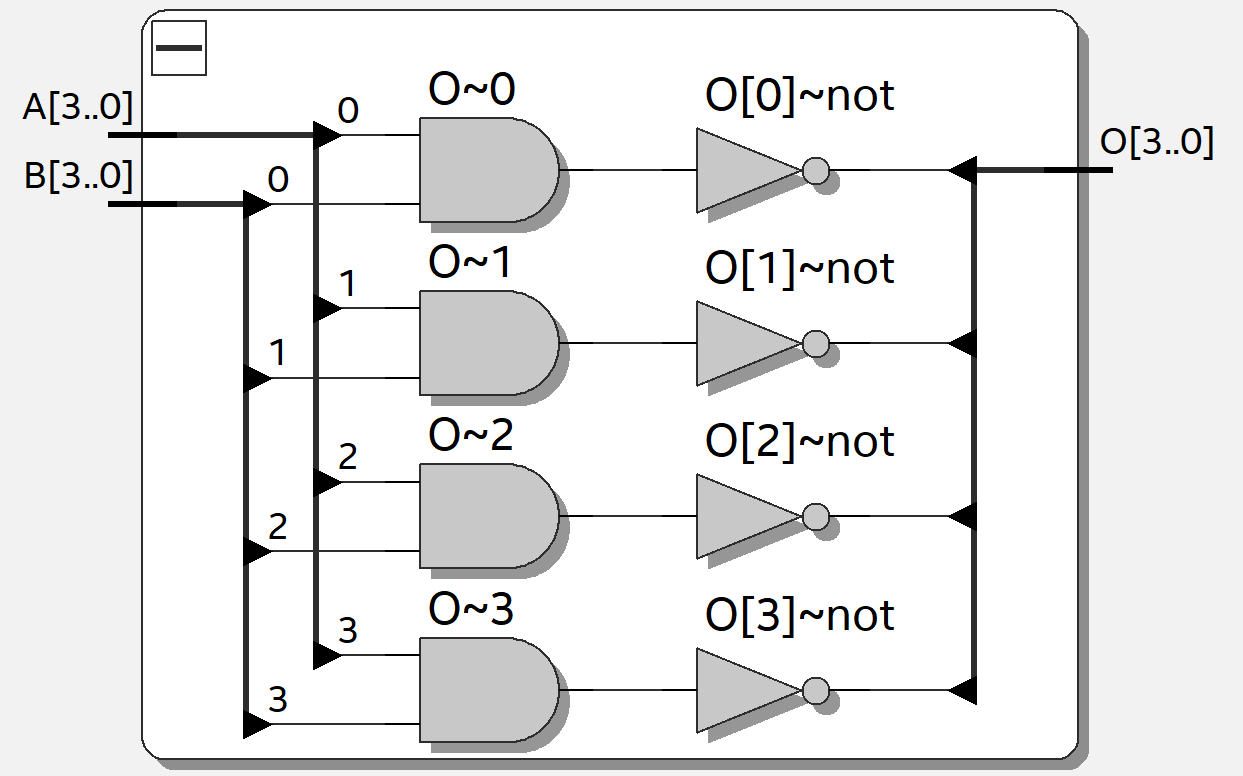
\includegraphics[scale=0.22]{Análise e Projeto/images/NAND.png}
            \tcbitem[squeezed title=Módulo \textit{MUX (LU)},center title,halign=center,valign=center]
                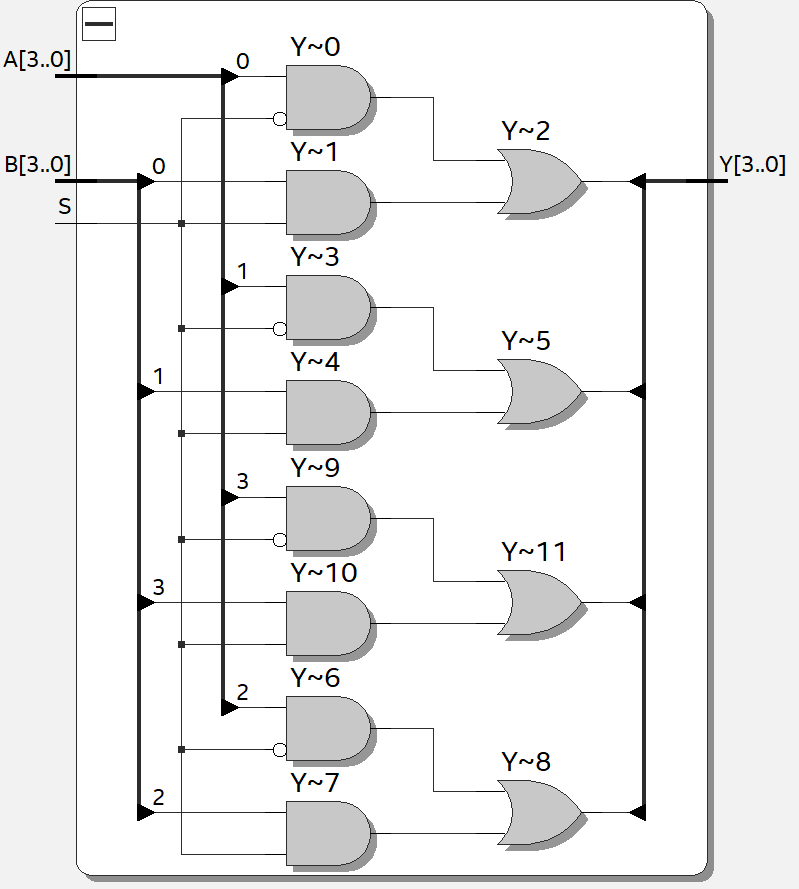
\includegraphics[scale=0.25]{Análise e Projeto/images/MUX Module.png}
        \end{tcbitemize}
    \end{tcolorbox}
    \caption{Sub-Módulos do Módulo Lógico}
\end{figure}
\newpage

\vspace*{\fill}
\begin{multicols}{2}
    \begin{inparaenum}[]
        \item{\begin{figure}[H]
                    \Subsubsec{\Centering Módulo de \textit{Flags}}
                    \centering
                    \tcbox[title=Módulo \textit{FLAGS},center title,halign=center,valign=center]{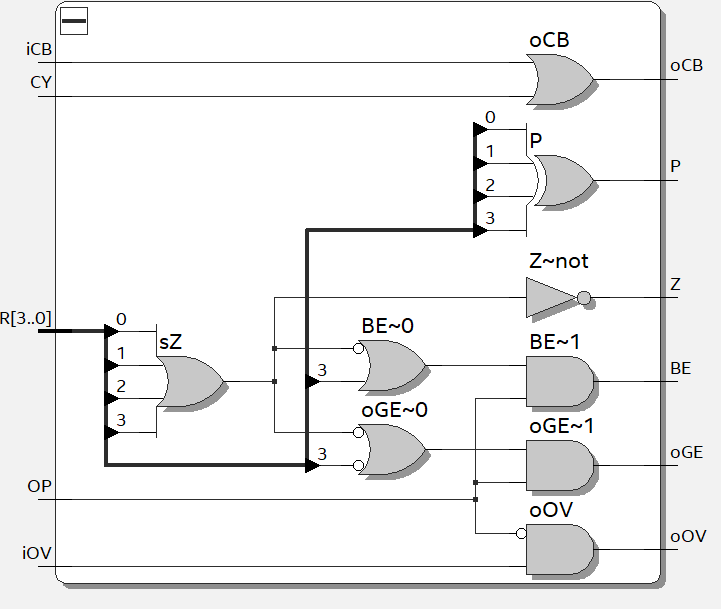
\includegraphics[scale=0.345]{Análise e Projeto/images/Flags Module.png}}
                    \caption{\Centering Diagrama lógico do Módulo \textit{FLAGS}}
                \end{figure}}\qquad
                
        \item{\begin{figure}[H]
                    \Subsubsec{\Centering Módulo \textit{Decoder}}
                    \centering
                    \tcbox[title=Módulo \textit{DECODER},center title,halign=center,valign=center]{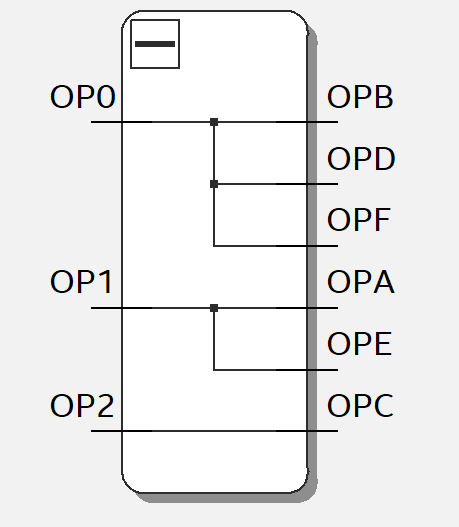
\includegraphics[scale=0.4]{Análise e Projeto/images/Decoder Module.png}}
                    \caption{\Centering Diagrama lógico do Módulo \textit{DECODER}}
                \end{figure}}
    \end{inparaenum}
\end{multicols}

\Subsubsec{Módulo MUX (ALU)}

\begin{figure}[H]
    \centering
    \tcbox[title=Módulo MUX (ALU),center title,halign=center,valign=center]{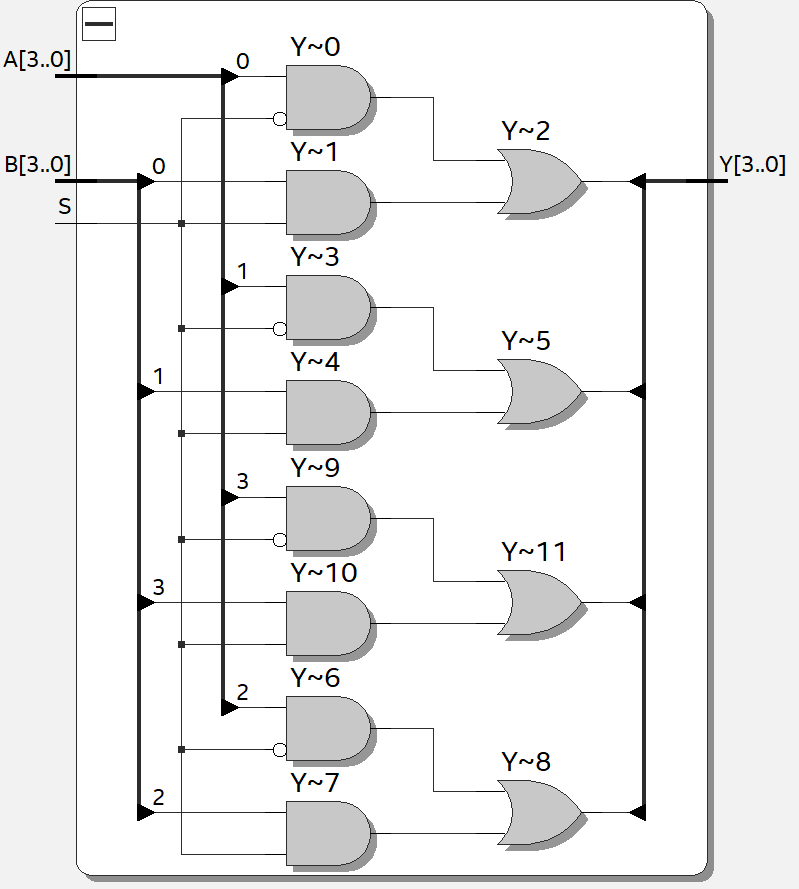
\includegraphics[scale=0.35]{Análise e Projeto/images/MUX Module.png}}
    \caption{Diagrama lógico do Módulo MUX (ALU)}
\end{figure}
\vspace*{\fill}%

\newpage

\Subsubsec{Módulo Y\textit{or0}}

\begin{figure}[H]
    \centering
    \tcbox[title=Módulo Y\textit{or}0,center title,halign=center,valign=center]{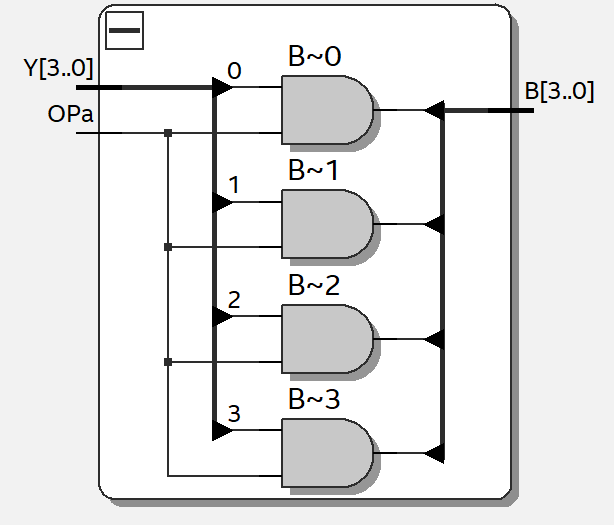
\includegraphics[scale=0.55]{Análise e Projeto/images/Yor0 Module.png}}
    \caption{Diagrama lógico do Módulo Y\textit{or}0}
\end{figure}

\vspace*{\fill}
\Subsubsec{ALU (Entidade Topo)}

\begin{figure}[H]
    \centering
    \tcbox[title=Diagrama completo (ALU),center title,halign=center,valign=center]{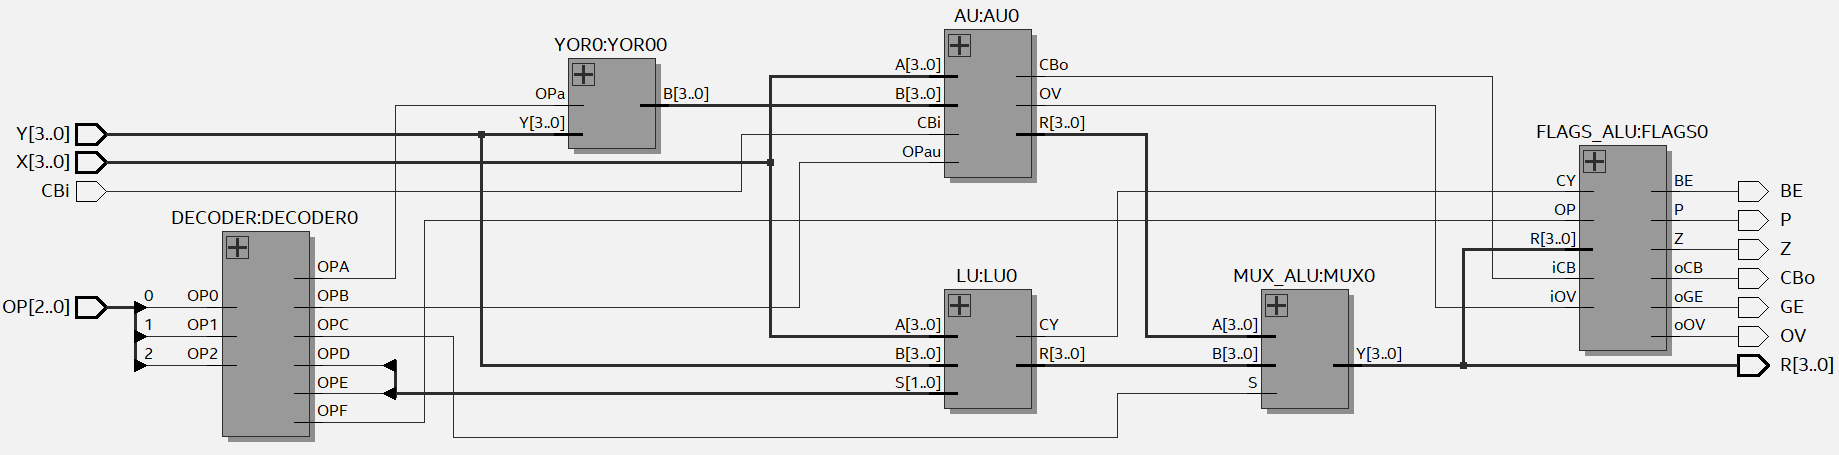
\includegraphics[scale=0.34]{Análise e Projeto/images/ALU Diagrama.png}}
    \caption{Diagrama lógico da ALU}
\end{figure}
\vspace*{\fill}%
\newpage